\chapter{Christ Judges the World (8:1--9:21)}

When the seventh seal\index{seals, seven!7@seventh seal} was opened, heaven fell silent for about half an hour (8:1). In that solemn stillness, John saw seven angels standing before God, each receiving a trumpet. The silence was the hush before judgment\index{judgment}, as though all heaven held its breath before the first trumpet\index{trumpets, seven!1@first trumpet} sounded.

Then the seven trumpets\index{trumpets, seven} sounded in succession. The first four struck the earth, the sea, the rivers, and the heavenly bodies. The fifth and sixth brought their terrors directly upon humanity. As the final three trumpets approached, an eagle flying overhead cried out, “Woe\index{woes, three}! Woe! Woe!” The threefold warning revealed the dreadful severity of the judgments still to come.\footnote{See Kuo, Chris \textit{The Eyes of the Eagle: See the Glory}, ISBN 979-8-9907810-9-2, https://drdataman01-ai.github.io/eagle-en-game/.}

Yet one detail deserves our careful attention: again and again, these judgments are limited to a third. Severe as they are, God's judgments remain restrained. He does not yet destroy the whole of creation; a measure of the world remains, and with it, room for repentance\index{repentance}. What is most astonishing, however, is that even after such devastation, humanity still refuses to repent (9:20--21).

\section{Prayer Rises Before God Like Incense}\index{incense}

\begin{ScriptureBox}

\item[8:2] And I saw the seven angels who stand before God, and seven trumpets were given to them.

\item[8:3] Another angel, who had a golden censer, came and stood at the altar. He was given much incense to offer, with the prayers of all God's people, on the golden altar in front of the throne.

\item[8:4] The smoke of the incense, together with the prayers of God's people, went up before God from the angel's hand.

\item[8:5] Then the angel took the censer, filled it with fire from the altar, and hurled it on the earth; and there came peals of thunder, rumblings, flashes of lightning and an earthquake.

\item[8:6] Then the seven angels who had the seven trumpets prepared to sound them.

\end{ScriptureBox}

God listens attentively to the prayers of His people. Their prayers rise before Him like fragrant incense\index{incense}, curling upward until they reach His presence. Prayer is not lost in the silence of heaven, nor does it vanish into the emptiness of suffering. God hears.

Throughout the Old Testament, incense\index{incense} serves as a powerful image of prayer. Psalm 141:2 expresses this longing: “May my prayer be set before you like incense”. Exodus 30:1--8 describes the altar\index{altar} of incense and the priestly service associated with it, while Leviticus 16:12--13 recounts the ritual in which incense was brought before the Lord. These practices belonged to Israel\index{Israel}'s worship\index{worship} in the earthly sanctuary.

In Revelation 8:3--4, the golden altar\index{altar} of incense\index{incense} appears within the heavenly scene. The imagery of the earthly tabernacle now opens a window into heavenly worship: the prayers of the saints rise before God's throne\index{throne of God}, received in His presence. Before the trumpets of judgment sound, heaven reveals something essential to the suffering church—God has not overlooked the prayers of His people.

Then the angel fills the censer with fire from the altar\index{altar} and hurls it upon the earth. Thunder, rumblings, flashes of lightning, and an earthquake\index{earthquake} follow. The prayers of the saints and the judgments of God are thus brought together in a solemn vision. The church's cries are not forgotten; justice belongs to the Lord, and the execution of judgment rests in His hands.

\begin{ReaderQuestion}
In Revelation 8:3--4, the prayers of the saints rise before God like incense. What does this image mean to you? When you have prayed for a long time without seeing any change, how might this passage help you trust that God has heard you?
\end{ReaderQuestion}

\section{The First Trumpet}\index{trumpets, seven!1@first trumpet}

\begin{ScriptureBox}

% Insert the licensed NIV text of Revelation 8:7.
\item[8:7] \textit{The first angel sounded his trumpet, and there came hail and fire mixed with blood, and it was hurled down on the earth. A third of the earth was burned up, a third of the trees were burned up, and all the green grass was burned up.}

\end{ScriptureBox}

\begin{figure}[htbp]
    \centering
    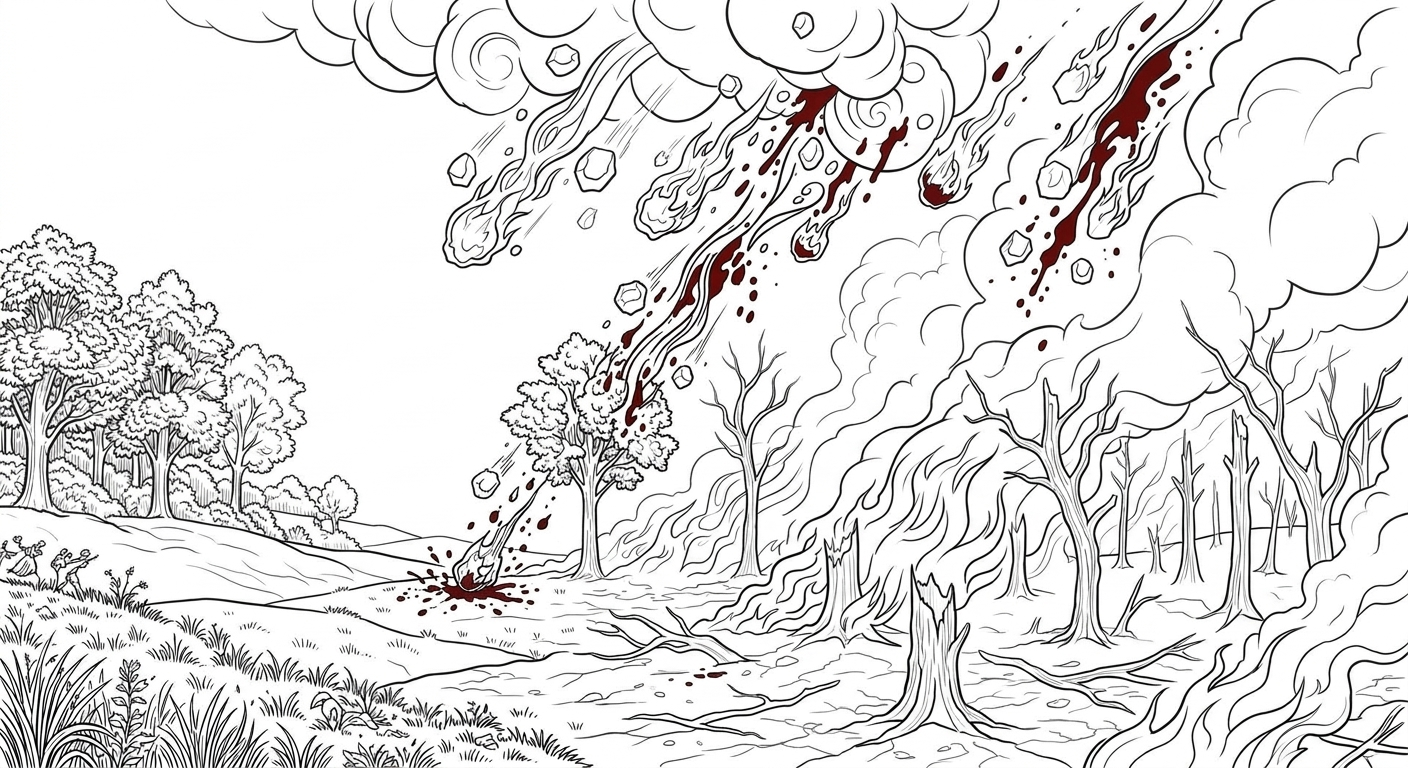
\includegraphics[
    width=1\textwidth,
    trim=0 0 0 0,
    clip]{images/trumpet_1st.jpg}
\end{figure}

At the sound of the first trumpet\index{trumpets, seven!1@first trumpet}, hail and fire mixed with blood are hurled upon the earth. A third of the earth is burned, along with a third of the trees and all the green grass.

The judgment begins with the land itself. What once nourished life is struck, and the familiar landscape becomes a scene of devastation. The green world, which bears witness to the Creator\index{Creator}'s generosity, now bears the marks of divine judgment. Yet the destruction is limited: a third is struck, not the whole.

\section{The Second Trumpet}\index{trumpets, seven!2@second trumpet}

\begin{ScriptureBox}

\item[8:8] The second angel sounded his trumpet, and something like a huge mountain, all ablaze, was thrown into the sea. A third of the sea turned into blood,

\item[8:9] a third of the living creatures in the sea died, and a third of the ships were destroyed.
% CHECK NIV: Revelation 8:8--9 supplied from memory, not from pasted text;
% verify wording against Bible Gateway (NIV 2011).

\end{ScriptureBox}

\begin{figure}[htbp]
    \centering
    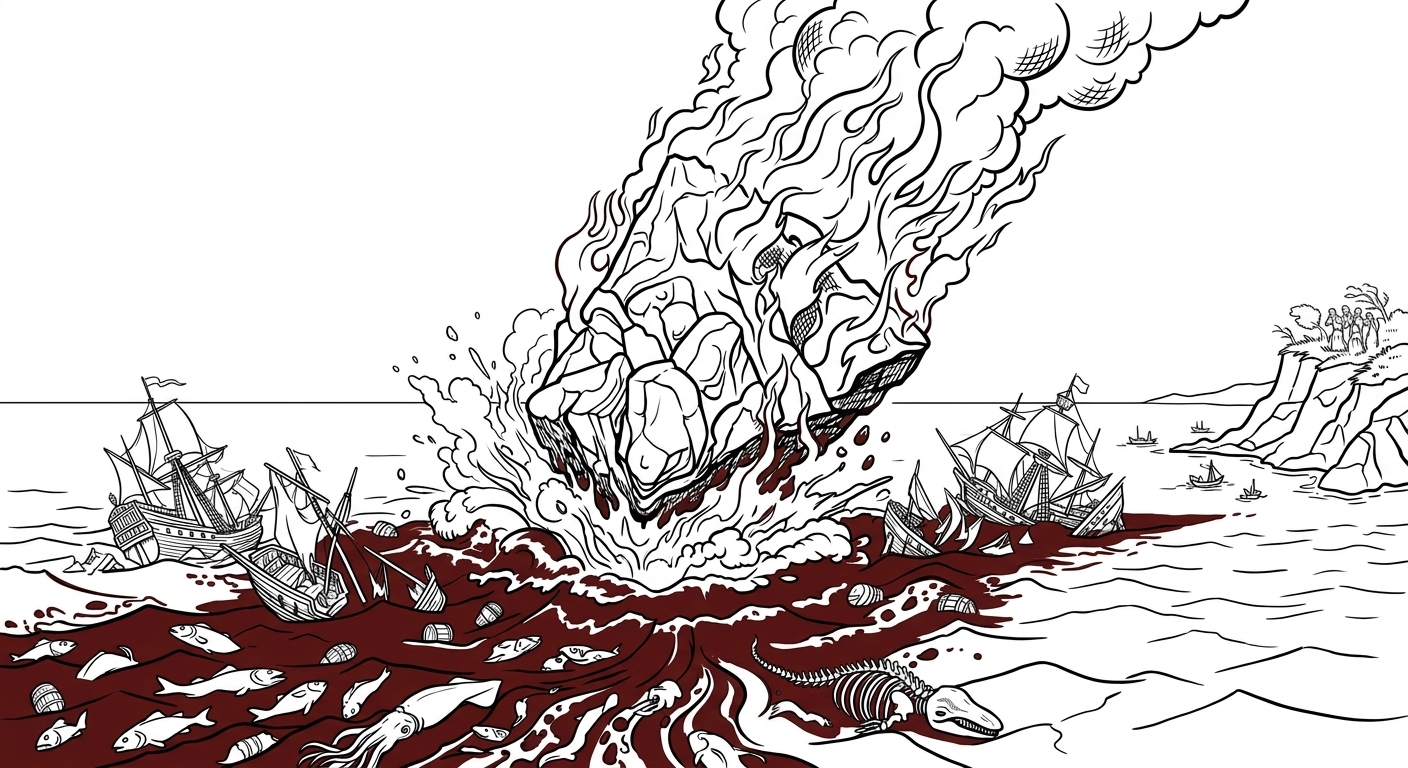
\includegraphics[
    width=1\textwidth,
    trim=0 0 0 0,
    clip]{images/trumpet_2nd.jpg}
\end{figure}

At the second trumpet\index{trumpets, seven!2@second trumpet}, something like a great mountain ablaze with fire is hurled into the sea. A third of the sea turns to blood, a third of its living creatures die, and a third of the ships are destroyed.

The sea, a source of food, commerce, and passage between distant lands, becomes a place of death and ruin. The destruction reaches beyond the shoreline, striking the creatures that inhabit the waters and the vessels that carry human life and trade across them. The judgment touches not only the natural world but also the networks upon which human civilization depends.

\section{The Third Trumpet}\index{trumpets, seven!3@third trumpet}

\begin{ScriptureBox}

\item[8:10] The third angel sounded his trumpet, and a great star, blazing like a torch, fell from the sky on a third of the rivers and on the springs of water---

\item[8:11] the name of the star is Wormwood. A third of the waters turned bitter, and many people died from the waters that had become bitter.
% NIV footnote for 8:11 (omitted; add as \footnote if wanted):
%   ``Wormwood'' --- Wormwood is a bitter substance.
% CHECK NIV: footnote wording quoted from memory; verify against Bible Gateway.

\end{ScriptureBox}

\begin{figure}[htbp]
    \centering
    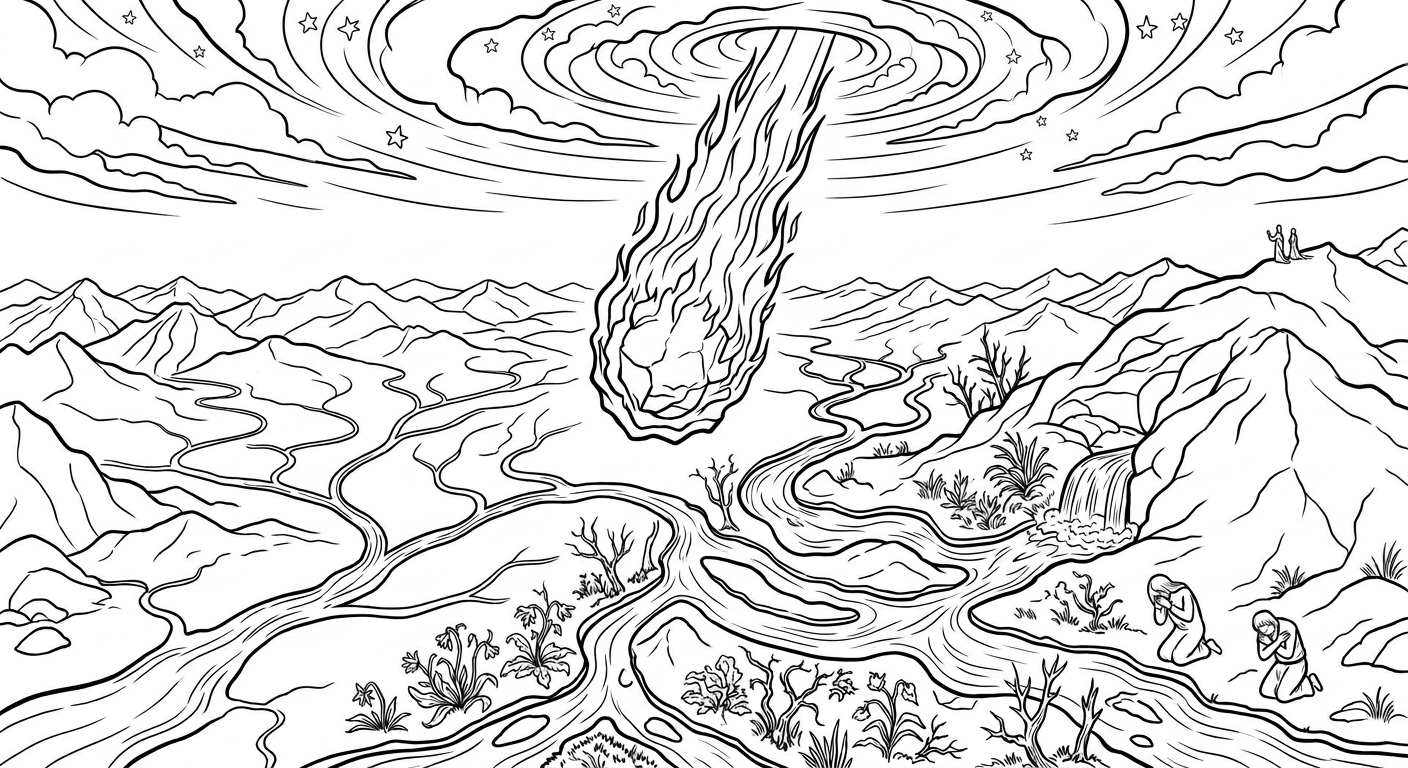
\includegraphics[
    width=1\textwidth,
    trim=0 0 0 0,
    clip]{images/trumpet_3rd.jpg}
\end{figure}

The star that falls from heaven is called Wormwood\index{Wormwood}. In Greek, the name is \textit{apsinthos}; in English, the plant is known as wormwood. It is associated with an intensely bitter taste. In the ancient world, wormwood was used for medicinal purposes and to repel insects; a related plant later became associated with the production of absinthe.

In the Old Testament, wormwood is often a symbol of bitterness, suffering, and judgment. Jeremiah 9:15, for example, declares that the people will be made to eat wormwood and drink poisoned water. Similar imagery appears in Lamentations 3:15 and Amos 5:7.

The vision in Revelation draws upon this established biblical imagery. When a third of the waters becomes wormwood, the emphasis falls on their bitter, undrinkable condition and the death that follows. Water, ordinarily a source of life, becomes an instrument of judgment. The very thing upon which human beings depend for survival is turned into a source of bitterness and death.

\section{The Fourth Trumpet}\index{trumpets, seven!4@fourth trumpet}

\begin{ScriptureBox}

% Insert the licensed NIV text of Revelation 8:12.
\item[8:12] \textit{The fourth angel sounded his trumpet, and a third of the sun was struck, a third of the moon, and a third of the stars, so that a third of them turned dark. A third of the day was without light, and also a third of the night.}

\end{ScriptureBox}

\begin{figure}[htbp]
    \centering
    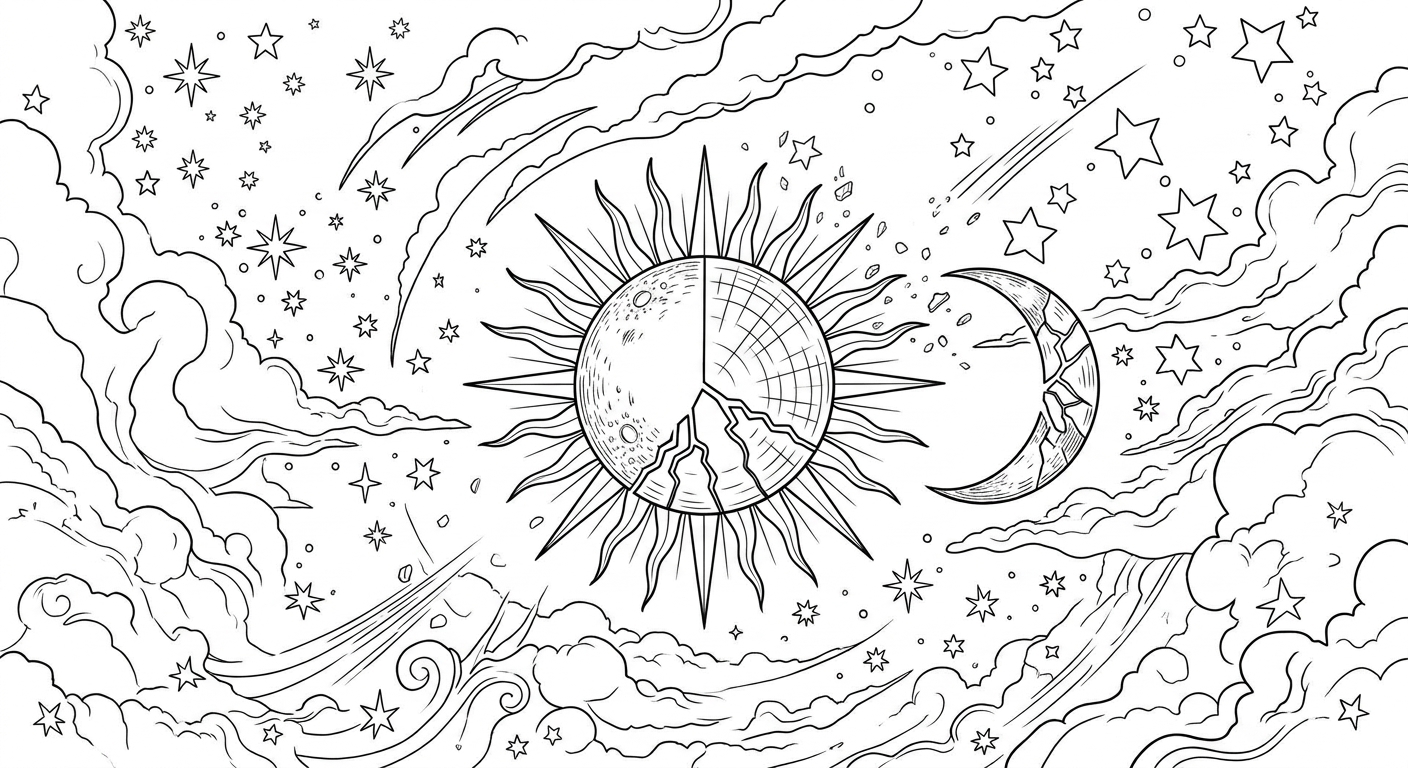
\includegraphics[
    width=1\textwidth,
    trim=0 0 0 0,
    clip]{images/trumpet_4th.jpg}
\end{figure}

At the fourth trumpet\index{trumpets, seven!4@fourth trumpet}, a third of the sun, moon, and stars is struck. A third of the day loses its light, and the night is darkened as well.

The rhythm of day and night, so familiar that humanity often takes it for granted, is disrupted. The lights that govern the heavens and mark the passage of time are darkened. The world below is left under a shadow that reaches from the earth to the sky.

The first four trumpets thus strike different parts of the created order: the land, the sea, the fresh waters, and the heavenly lights. Yet each judgment remains partial. The repeated limitation to a third is a sobering reminder that the devastation is real, but the final destruction has not yet come.

\section{The Fifth Trumpet}\index{trumpets, seven!5@fifth trumpet}

\begin{ScriptureBox}

\item[8:13] \textit{As I watched, I heard an eagle that was flying in midair call out in a loud voice: “Woe! Woe! Woe to the inhabitants of the earth, because of the trumpet blasts about to be sounded by the other three angels!”}

\item[9:1] The fifth angel sounded his trumpet, and I saw a star that had fallen from the sky to the earth. The star was given the key to the shaft of the Abyss.

\item[9:2] When he opened the Abyss, smoke rose from it like the smoke from a gigantic furnace. The sun and sky were darkened by the smoke from the Abyss.

\item[9:3] And out of the smoke locusts came down on the earth and were given power like that of scorpions of the earth.

\item[9:4] They were told not to harm the grass of the earth or any plant or tree, but only those people who did not have the seal of God on their foreheads.

\item[9:5] They were not allowed to kill them but only to torture them for five months. And the agony they suffered was like that of the sting of a scorpion when it strikes.

\item[9:6] During those days people will seek death but will not find it; they will long to die, but death will elude them.

\item[9:7] The locusts looked like horses prepared for battle. On their heads they wore something like crowns of gold, and their faces resembled human faces.

\item[9:8] Their hair was like women's hair, and their teeth were like lions' teeth.

\item[9:9] They had breastplates like breastplates of iron, and the sound of their wings was like the thundering of many horses and chariots rushing into battle.

\item[9:10] They had tails with stingers, like scorpions, and in their tails they had power to torment people for five months.

\item[9:11] They had as king over them the angel of the Abyss, whose name in Hebrew is Abaddon and in Greek is Apollyon (that is, Destroyer).

\item[9:12] The first woe is past; two other woes are yet to come.

\end{ScriptureBox}

\begin{figure}[htbp]
    \centering
    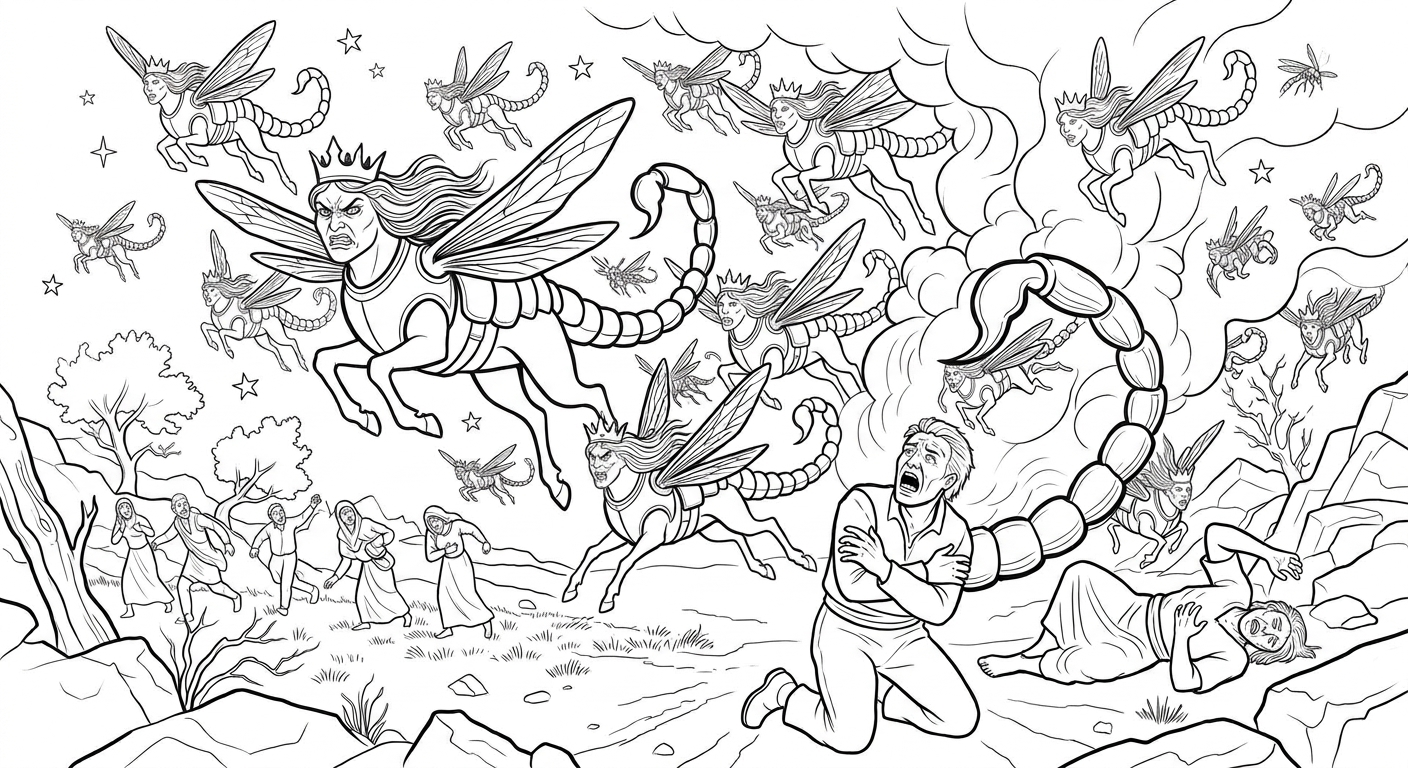
\includegraphics[
    width=1\textwidth,
    trim=0 0 0 0,
    clip]{images/trumpet_5th.jpg}
\end{figure}

As the first four trumpets fall silent, John sees an eagle flying overhead, proclaiming three woes\index{woes, three} upon the inhabitants of the earth. The remaining trumpets will bring judgments of a different and more terrifying kind. The first woe begins when the fifth angel sounds his trumpet.

A star has fallen from heaven to earth, and the key to the Abyss\index{Abyss} is given to it. When the Abyss is opened, smoke rises like the smoke of a great furnace, darkening the sun and the sky. Out of the smoke comes a swarm of locusts\index{locusts}, but these are no ordinary insects. They are granted power like that of scorpions, and their mission is unlike that of the locusts familiar to the world.

They are forbidden to harm the grass, plants, or trees. Instead, they are commanded to torment those who do not bear the seal of God on their foreheads. They cannot kill their victims, but for five months they inflict agony like the sting of a scorpion. The suffering is so severe that people long for death, yet death eludes them.

John describes the locusts\index{locusts} through a succession of startling comparisons. They resemble horses prepared for battle, wear something like crowns of gold, and have faces like human faces. Their hair is like women's hair, their teeth like lions' teeth, and their breastplates like iron. The sound of their wings resembles the thunderous rush of chariots and horses charging into battle. Their tails are like scorpions, armed with stingers that torment people for five months.

Their king is the angel of the Abyss\index{Abyss}, called Abaddon in Hebrew and Apollyon in Greek—names associated with destruction and the destroyer. The first woe has passed, but two more are still to come.

The vision is terrifying not merely because it depicts strange and dreadful creatures, but because it portrays a realm of judgment in which torment is permitted yet bounded. The locusts\index{locusts} can harm, but they cannot kill; their power is real, but it is limited. Even in the midst of this darkness, the vision continues to reveal that evil does not exercise unlimited authority.

\section{The Sixth Trumpet}\index{trumpets, seven!6@sixth trumpet}

\begin{ScriptureBox}

\item[9:13] The sixth angel sounded his trumpet, and I heard a voice coming from the four horns of the golden altar that is before God.

\item[9:14] It said to the sixth angel who had the trumpet, ``Release the four angels who are bound at the great river Euphrates.''

\item[9:15] And the four angels who had been kept ready for this very hour and day and month and year were released to kill a third of mankind.

\item[9:16] The number of the mounted troops was twice ten thousand times ten thousand. I heard their number.

\item[9:17] The horses and riders I saw in my vision looked like this: Their breastplates were fiery red, dark blue, and yellow as sulfur. The heads of the horses resembled the heads of lions, and out of their mouths came fire, smoke and sulfur.

\item[9:18] A third of mankind was killed by the three plagues of fire, smoke and sulfur that came out of their mouths.

\item[9:19] The power of the horses was in their mouths and in their tails; for their tails were like snakes, having heads with which they inflict injury.

\item[9:20] The rest of mankind who were not killed by these plagues still did not repent of the work of their hands; they did not stop worshiping demons, and idols of gold, silver, bronze, stone and wood---idols that cannot see or hear or walk.

\item[9:21] Nor did they repent of their murders, their magic arts, their sexual immorality or their thefts.

\end{ScriptureBox}

\begin{figure}[htbp]
    \centering
    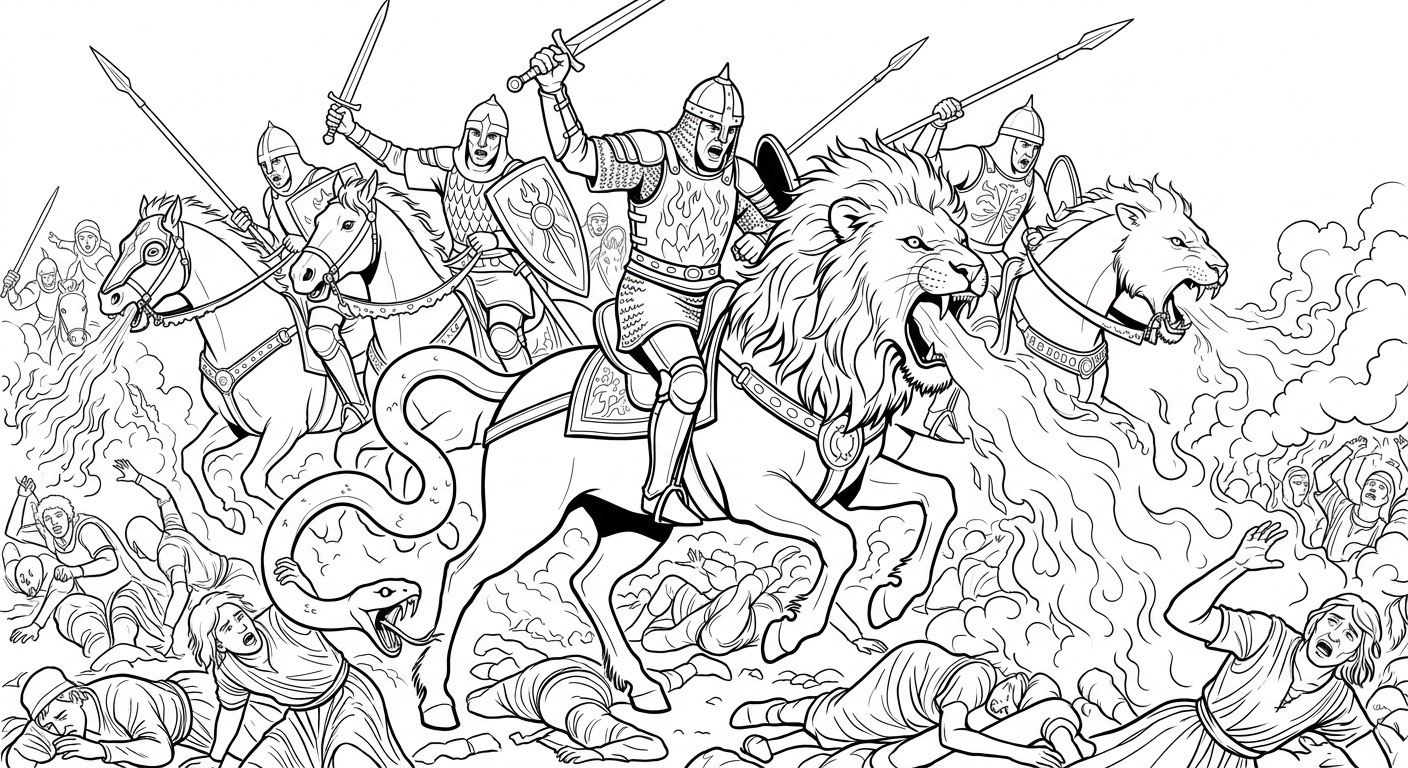
\includegraphics[
    width=1\textwidth,
    trim=0 0 0 0,
    clip]{images/trumpet_6th.jpg}
\end{figure}

When the sixth angel sounds his trumpet, a voice comes from the four horns of the golden altar\index{altar} before God. The angel is commanded to release the four angels bound at the great river Euphrates\index{Euphrates}. They have been kept ready for a precise moment—the appointed year, month, day, and hour—when they will kill a third of humanity.

The four angels command an army of two hundred million horsemen. John hears their number and then sees them in his vision. The riders wear breastplates the color of fire, sapphire, and sulfur. The horses have heads like lions, and fire, smoke, and sulfur pour from their mouths. These three plagues\index{plagues} kill a third of humanity. The horses' power lies in their mouths and tails; their tails resemble snakes, with heads that inflict harm.

The identity of the four bound angels is not made explicit. They may represent fallen angels or demonic powers held in restraint, though some interpreters have also considered historical military forces. The vision's emphasis, however, is clear: a vast and terrifying force is released to bring death upon humanity, and its activity unfolds under a divinely appointed limit.

The expression “two hundred million” is often understood in light of the Greek wording, which conveys the idea of an immense number—literally, “myriads of myriads.” The image emphasizes the overwhelming scale of the army; it need not be treated as a modern statistical report calculated by multiplying twenty thousand by twenty thousand.

The Euphrates\index{Euphrates} was an important geographical boundary to the northeast of ancient Israel\index{Israel}. It was also associated with the territory promised by God and with the threat of foreign powers advancing from the northeast.\footnote{When God made His covenant with Abraham, He promised his descendants territory extending from the river of Egypt to the Euphrates (Genesis 15:18). Isaiah, meanwhile, used the image of the Euphrates overflowing its banks to portray the might of the king of Assyria and his armies, whose power would sweep into Judah like a flood (Isaiah 8:7--8).} In Revelation, the judgment associated with this river reaches beyond the borders of ancient Israel and touches humanity on a vast scale.

One might expect a calamity of such magnitude to bring people to repentance\index{repentance}. Yet disaster does not, by itself, produce a repentant heart. This is one of the most sobering truths in the passage. Even after witnessing death and devastation, the survivors refuse to turn from the works of their hands. They continue to worship demons and lifeless idols made of gold, silver, bronze, stone, and wood—things that cannot see, hear, or walk. They also refuse to repent of their murders, sorceries, sexual immorality, and theft.

The tragedy is not merely that humanity suffers judgment. It is that humanity persists in rebellion even while judgment unfolds before its eyes. The human heart can witness devastation and still cling to the very sins that lead to ruin.

\begin{ReaderQuestion}
Revelation 9:20--21 emphasizes that people still refuse to repent even after experiencing devastating judgments. Why do suffering and disaster not necessarily lead people to repentance? What does this passage teach us about the nature of repentance and the human heart?
\end{ReaderQuestion}

Once again, the repeated limitation to a third deserves attention. The judgments of the trumpets are severe, but they do not yet consume the whole created order. The world is struck, but not wholly destroyed. The restraint is significant: judgment has come, yet the vision has not reached the final end of all things.

\begin{figure}[htbp]
    \centering
    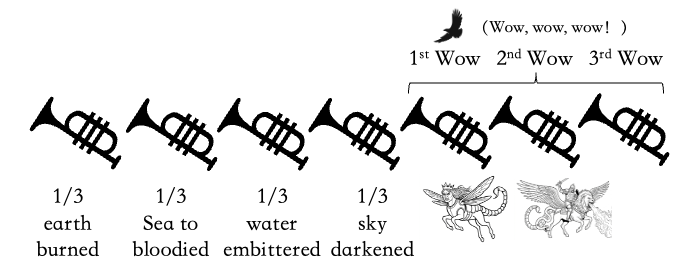
\includegraphics[
    width=1\textwidth,
    trim=0 0 0 0,
    clip]{images/trumpets_woes.png}
    \caption{The Seven Trumpets}
    \label{fig:trumpets_woes}
\end{figure}

\section{Future Events, Ancient Language}

You may have noticed that God allows John to describe these visions through images familiar to people of the first century: horses, cavalry, and the weapons of ancient warfare. Yet modern warfare no longer depends on horses and swords. It employs drones, fighter jets, missiles, and increasingly sophisticated military technologies. The wars of the future may involve technologies beyond anything we can presently imagine.

If the visions in Revelation concern future events, why does John describe them in terms of horses and ancient weapons? Why did God not simply show John the military technology of the future and enable him to describe it directly? Some readers have even suggested that the horses must be tanks, the fire must be missiles, or the locusts\index{locusts} must be helicopters.

A more careful answer is that God's purpose is not to give John a preview of future weapons technology. His purpose is to reveal His judgment and sovereignty. Seeing a future technology would not necessarily mean understanding the revelation God intended to communicate. God gave John visions in a form he could describe to the people of his own time, while preserving their significance for readers in generations to come.

Consider Revelation 9:7, which says that the locusts\index{locusts} looked like horses prepared for battle. Revelation 9:17 describes horses with heads like lions, and verse 19 compares their tails to snakes. John does not simply say, “I saw horses.” Again and again, he reaches for the words “like” and “as” to convey what he sees. His language is the language of comparison, attempting to express a vision that exceeds ordinary experience.

Imagine, for a moment, that God had shown John an F-35 fighter jet. How might a man of the first century have described it? He might have written, “I saw an enormous iron bird with two wings, breathing fire as it flew across the sky.” Such a description might sound strange to a modern reader, but it would be a natural attempt to convey an unfamiliar sight using familiar language.

Throughout Revelation, words such as “like” and “as” remind us that John is describing extraordinary visions through the language available to him. We should therefore be cautious about translating the imagery directly into modern military hardware, such as Apache helicopters or contemporary tanks. Such identifications may seem compelling in one generation and become obsolete in the next. More importantly, they can distract us from the theological message of the vision.\footnote{See G. K. Beale (1999) and Richard Bauckham (1993).}

There is another reason to resist reducing these images to modern technology: Revelation is deeply rooted in the language and imagery of the Old Testament. The locusts\index{locusts} in Revelation 9, for example, strongly recall Joel's prophecy of the day of the Lord\index{day of the Lord}. Joel 2:4 describes the locusts this way: “They have the appearance of horses; they gallop along like cavalry” (NIV).

Readers familiar with Israel\index{Israel}'s Scriptures would recognize this language and recall the prophetic themes associated with the day of the Lord\index{day of the Lord}, divine judgment, and the end of the age. The imagery in Revelation is not merely a coded description of some future weapon. It draws the reader into the larger biblical story of God's judgment against evil and His ultimate rule over history.

If John had instead described an F-35, his readers might have struggled to understand the image, and the connection to Joel's prophecy would have been obscured. By using the language of Scripture, the vision speaks across generations. Its central message does not depend on our ability to identify a particular machine or predict a particular military event. It calls us to recognize the seriousness of divine judgment, the limits of human power, and the need to turn to God in repentance\index{repentance}.

The eagle's task is therefore not to gaze into the vision merely to identify the machinery of war, but to look beyond the terrifying images and discern the truth they reveal: history remains under God's sovereign hand, judgment is real, and humanity's greatest need is not technological understanding but a heart willing to repent.
